% ==================== 2.3.2.5 金红石 ====================
\jiegou{2.3.2.5}{金红石结构（\texorpdfstring{TiO$_2$}{TiO2}）}

金红石型 TiO$_2$ 属四方晶系（$P\,4_2/m\,n\,m$，No.~136），建模输入值如表~\ref{tab:rutile}
所列。氧原子位于 $4f$ 位 $(x,x,0)$（$x\approx0.3$），表中列出的是模型中实际输入的
4 个等效氧原子坐标。

\begin{table}[H]
  \centering
  \caption{金红石（TiO$_2$）结构的建模参数}
  \label{tab:rutile}
  \begin{tabular}{ll}
    \toprule
    项目 & 参数 \\
    \midrule
    空间群 & $P\,4_2/m\,n\,m$（No.~136） \\
    晶格常数 & $a=b=4.6$\,\AA，$c=2.9634$\,\AA，$\alpha=\beta=\gamma=90^\circ$ \\
    原子坐标 & Ti：$(0,0,0)$、$(1/2,1/2,1/2)$（$2a$ 位）； \\
      & O：$(0.3,0.3,0)$、$(0.8,0.2,0.5)$； \\
      & O：$(0.7,0.7,0.5)$、$(0.2,0.8,0.5)$（$4f$ 位，$x\approx0.3$） \\
    化学式单元数 & $Z=2$ \\
    \bottomrule
  \end{tabular}
\end{table}

\begin{figure}[H]
  \centering
  \subcaptionbox{空间群与晶格常数设置}{%
    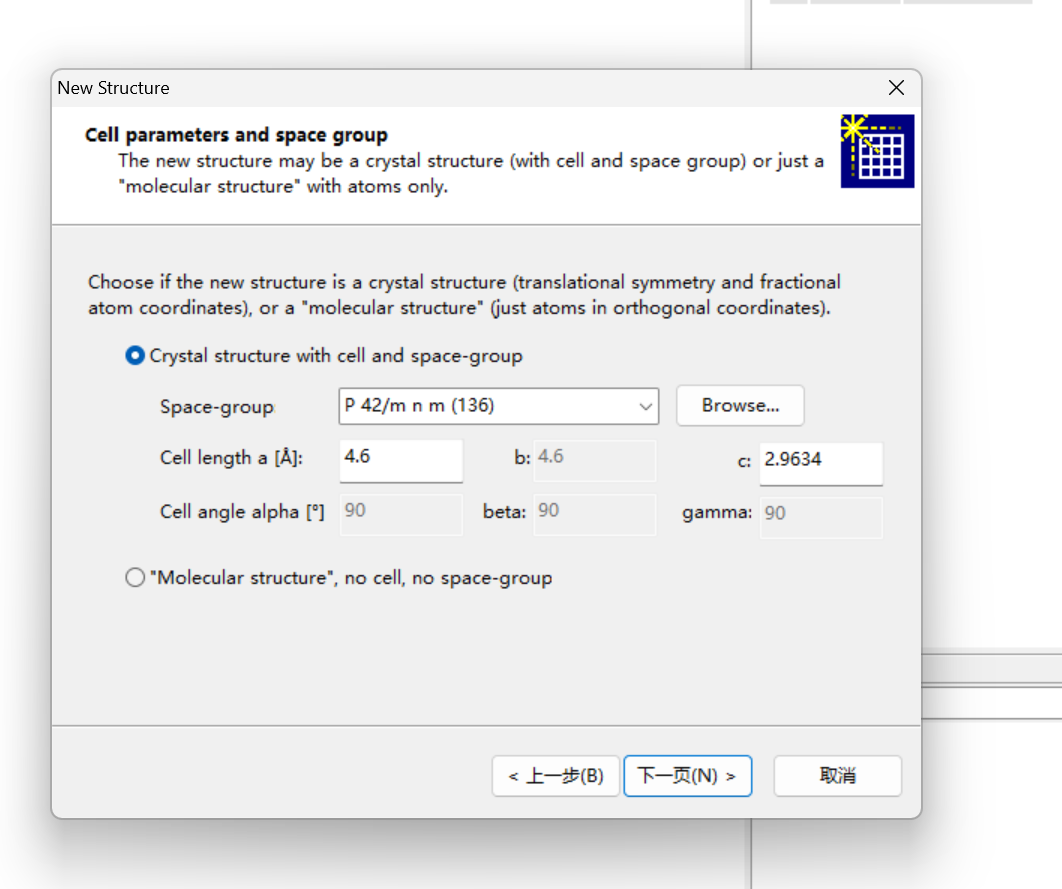
\includegraphics[width=0.44\textwidth]{assets/rutile/a.png}}
  \hfill
  \subcaptionbox{非对称单元原子（Ti、O）添加}{%
    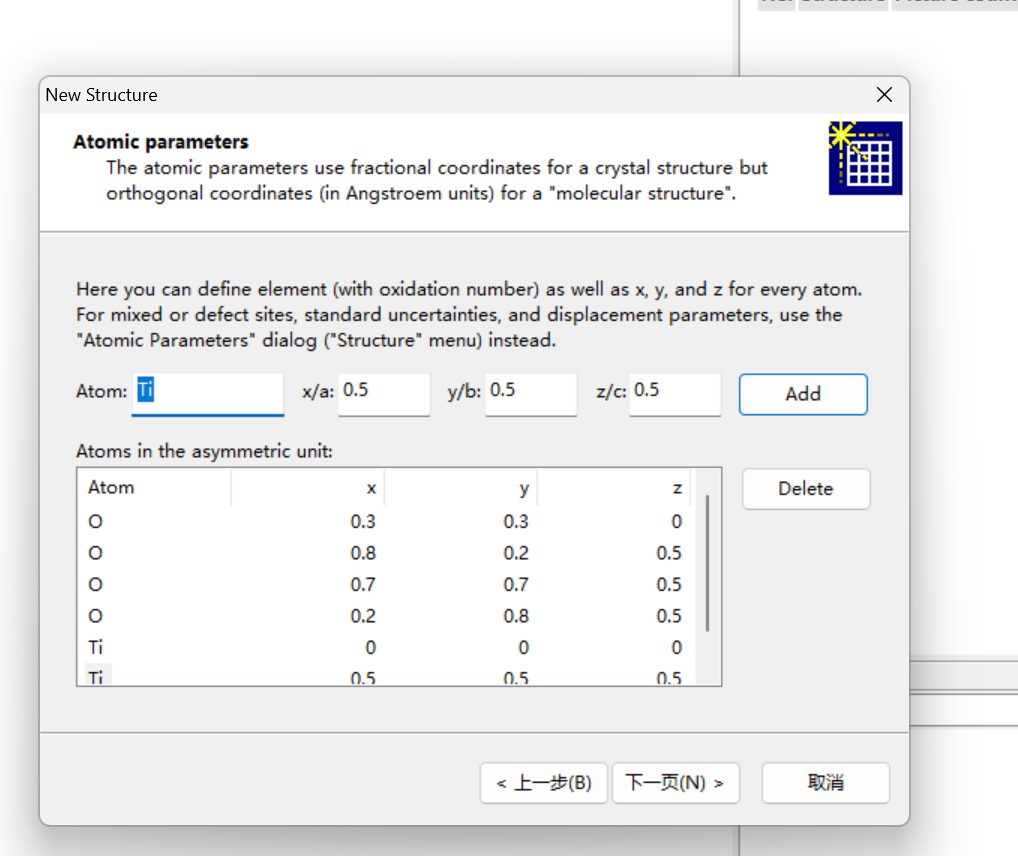
\includegraphics[width=0.44\textwidth]{assets/rutile/b.png}}
  \caption{金红石（TiO$_2$）结构的参数设置}
  \label{fig:rutile-param}
\end{figure}

\begin{figure}[H]
  \centering
  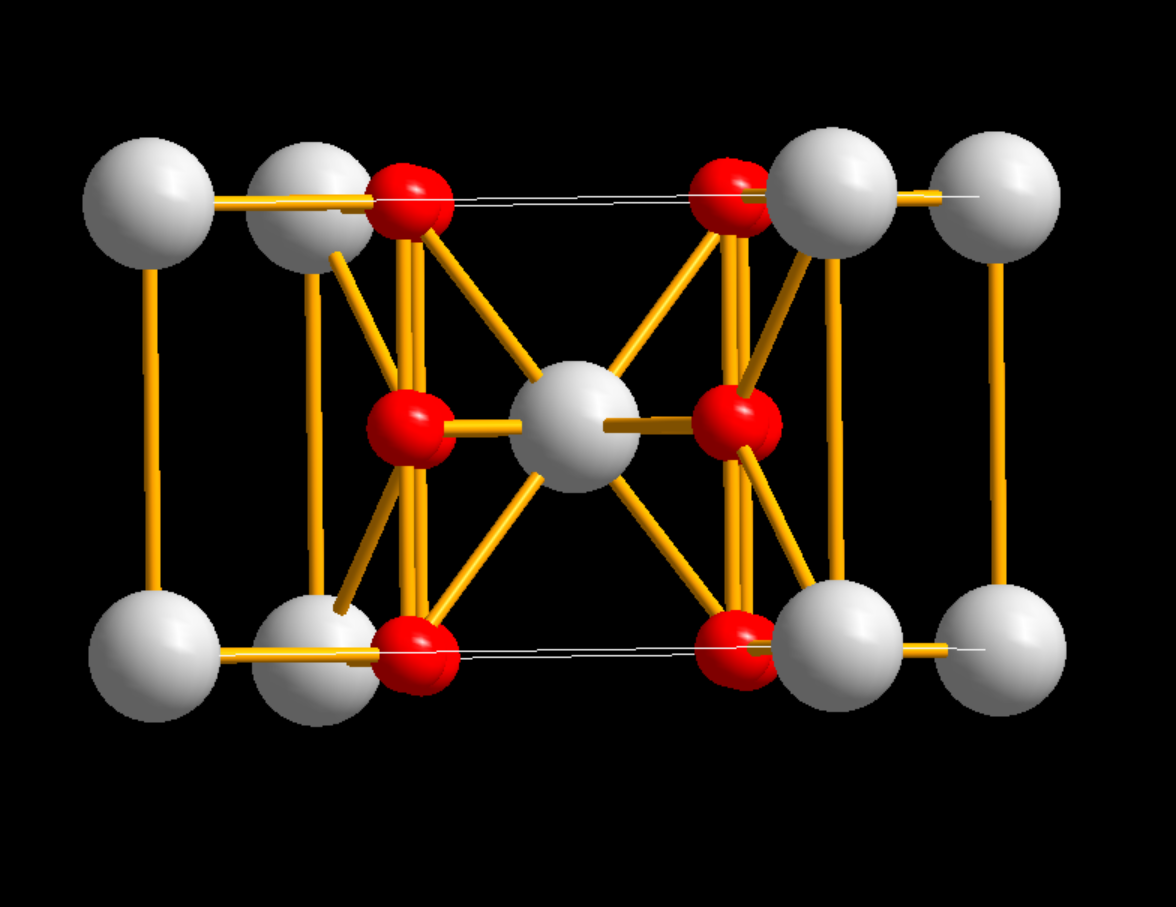
\includegraphics[width=0.5\textwidth]{assets/rutile/c.png}
  \caption{金红石（TiO$_2$）结构的晶体结构模型}
  \label{fig:rutile-model}
\end{figure}

\begin{figure}[H]
  \centering
  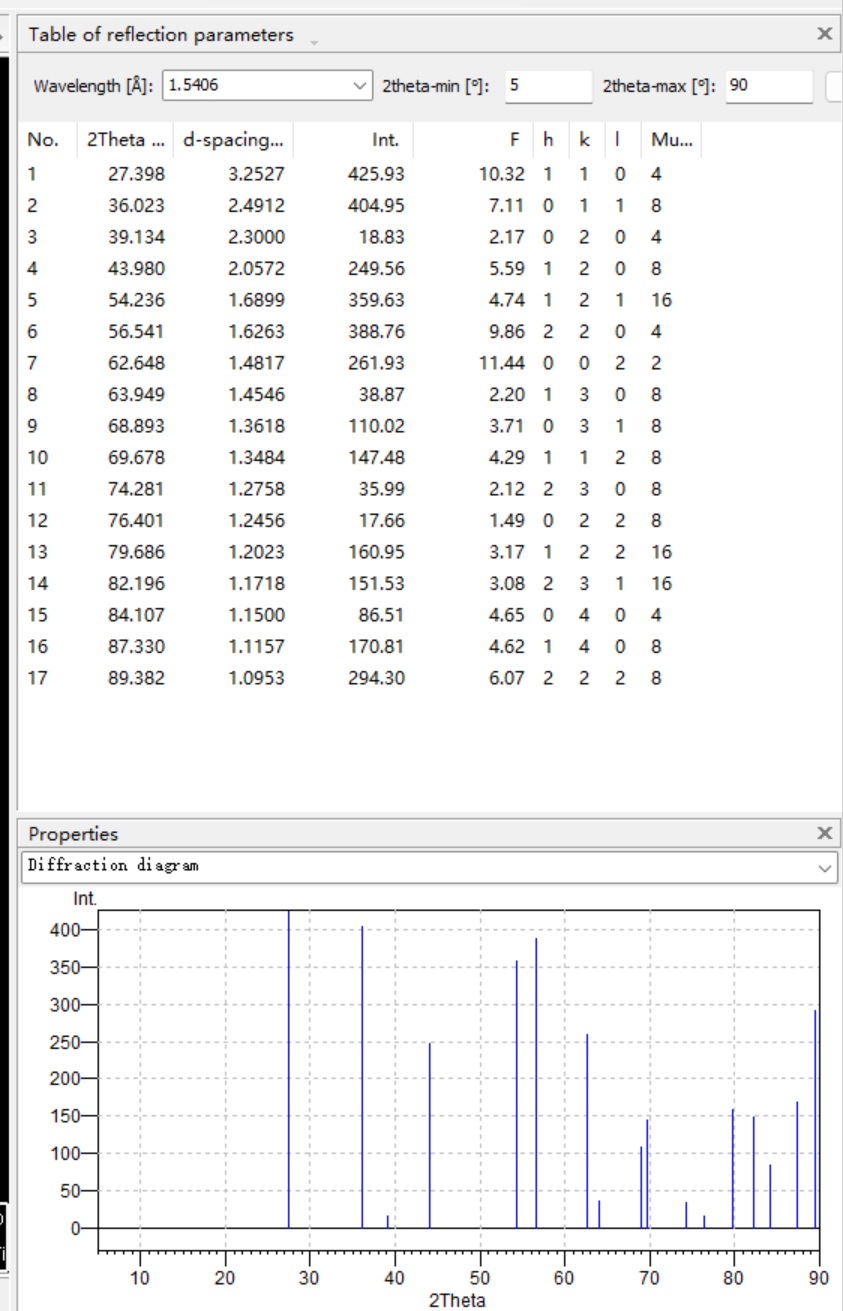
\includegraphics[width=0.4\textwidth]{assets/rutile/d.png}
  \caption{Diamond 模拟的金红石（TiO$_2$）结构粉末衍射图}
  \label{fig:rutile-xrd}
\end{figure}

\begin{figure}[H]
  \centering
  \subcaptionbox{晶面视图}{%
    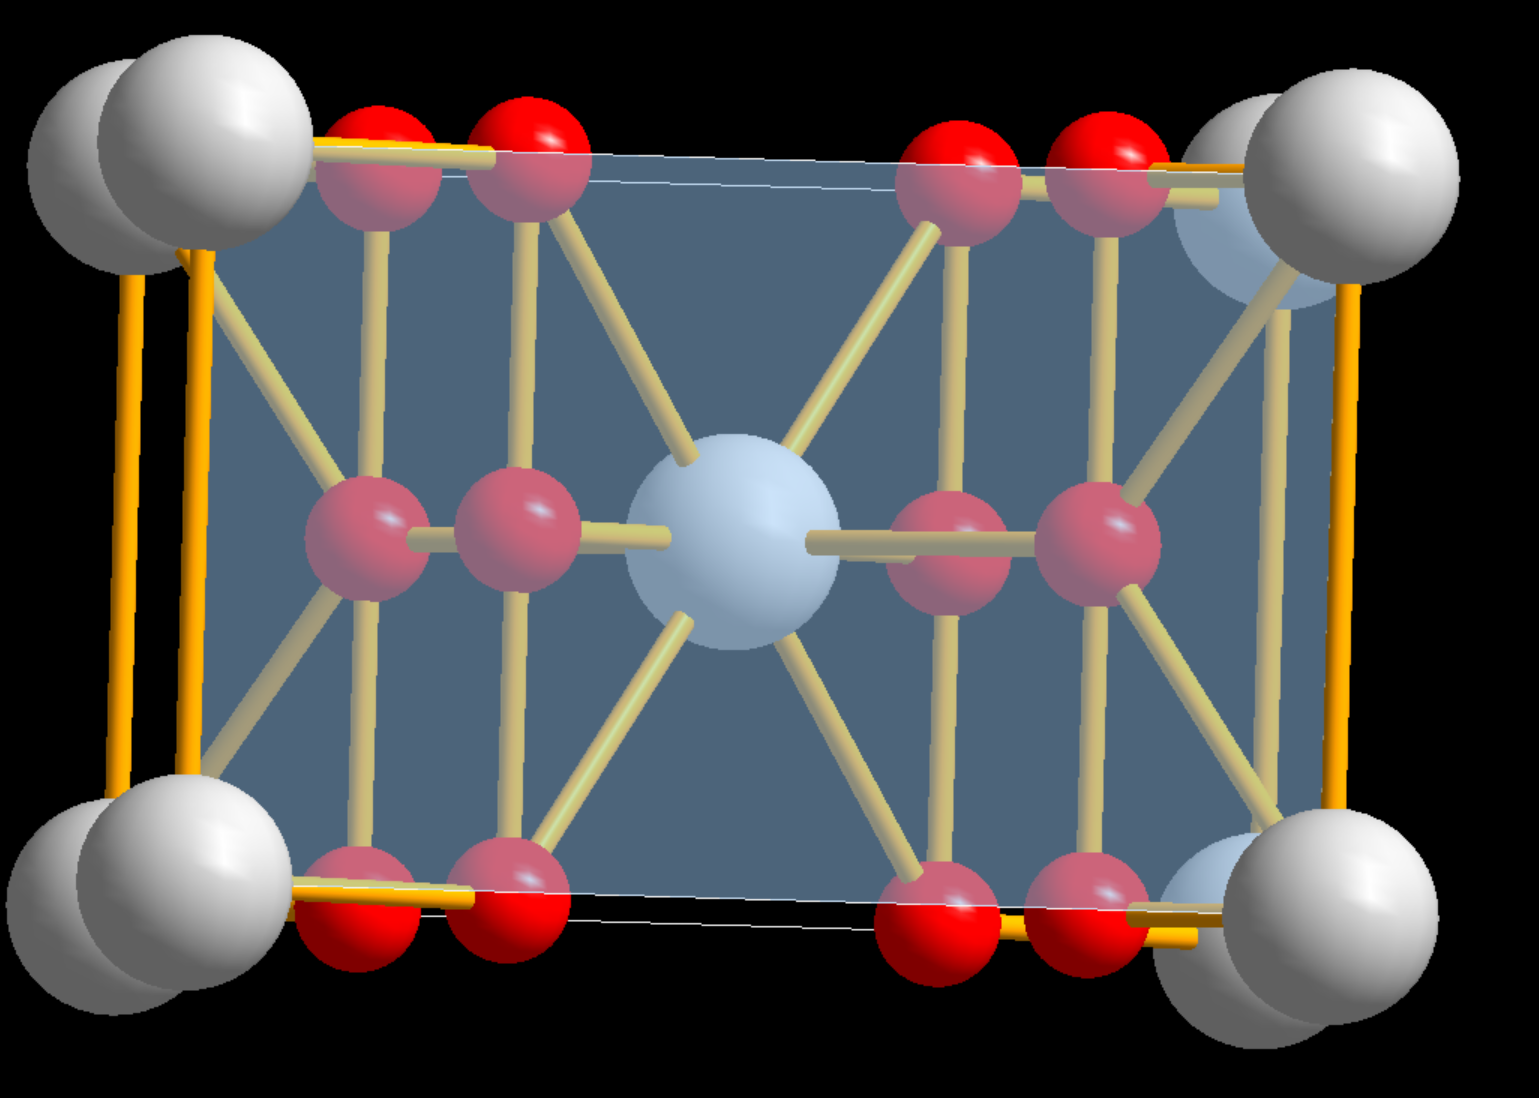
\includegraphics[width=0.44\textwidth]{assets/rutile/e.png}}
  \hfill
  \subcaptionbox{TiO$_6$ 配位八面体}{%
    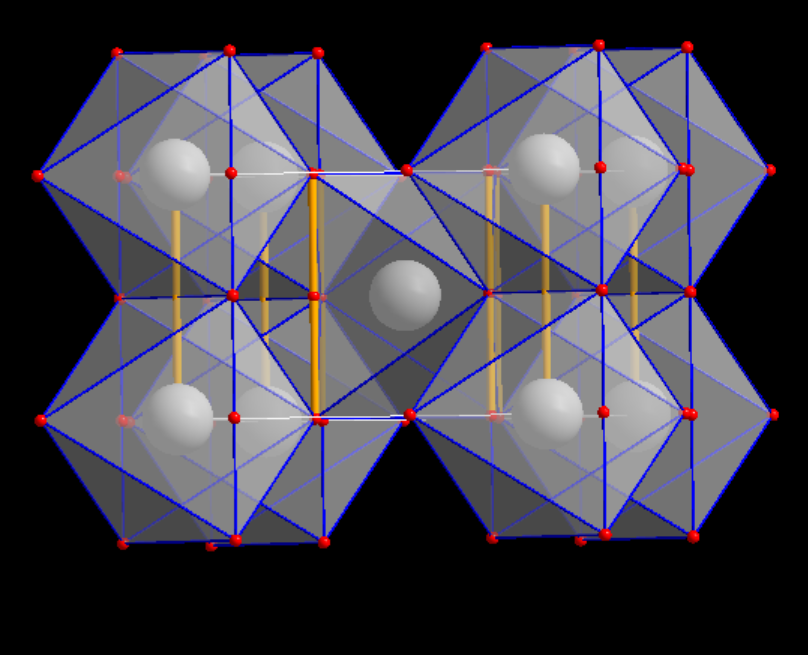
\includegraphics[width=0.28\textwidth]{assets/rutile/f.png}}
  \hfill
  \subcaptionbox{配位多面体设置}{%
    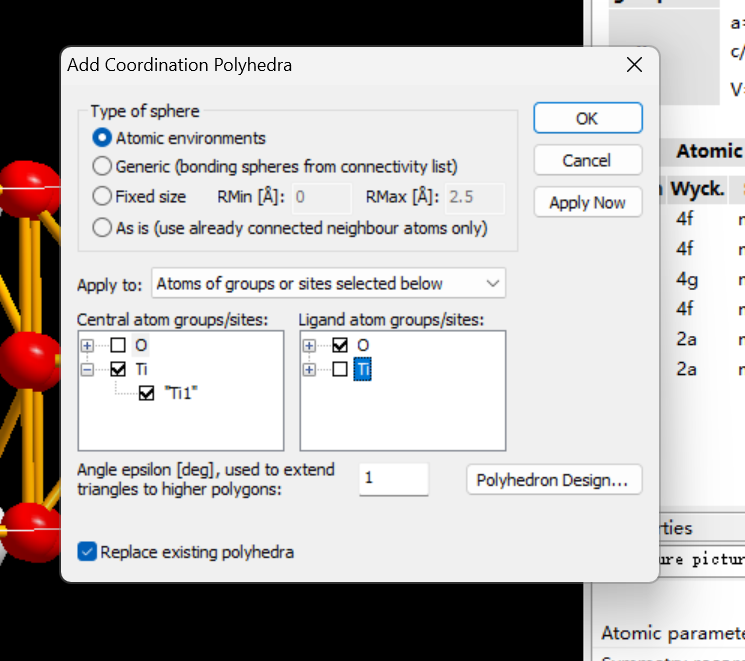
\includegraphics[width=0.24\textwidth]{assets/rutile/f1.png}}
  \caption{金红石（TiO$_2$）结构的晶面与配位八面体}
  \label{fig:rutile-plane}
\end{figure}

\textbf{结构特征。}每个 Ti$^{4+}$ 位于 TiO$_6$ 八面体中心，与 6 个 O$^{2-}$ 配位；
每个 O$^{2-}$ 反过来被 3 个 Ti$^{4+}$ 包围，呈平面三角配位。

把 $x=0.3$、$a=4.6$\,\AA、$c=2.9634$\,\AA 代入模型坐标，可以算出两类 Ti--O 键长：
赤道方向的 4 个键长为 $\sqrt{2}\,x\,a=\sqrt{2}\times0.3\times4.6\approx1.95$\,\AA；
顶点方向的 2 个键长为
\begin{equation}
  d_{\text{顶}}=\sqrt{2\bigl(\tfrac12-x\bigr)^2a^2+\frac{c^2}{4}}
    =\sqrt{2\times0.2^2\times4.6^2+2.9634^2/4}\approx1.97\ \text{\AA}
\end{equation}
八面体沿顶点方向被略微拉长。连接方式上，TiO$_6$ 八面体沿 $c$ 轴共棱连成无限链
（图~\ref{fig:rutile-plane}(b)），链与链之间再通过共用顶点（赤道氧）相连，构成三维
骨架；链内 Ti--Ti 距离因此较小，相邻链之间则靠共顶点氧联系。$P\,4_2/m\,n\,m$ 中
$4_2$ 螺旋轴沿 [001] 方向，$n$ 滑移面与镜面 $m$ 分别位于 [100]、[110] 方向，与
八面体链沿 $c$ 轴的螺旋排列相对应。

金红石相是常压下 TiO$_2$ 最稳定的晶型；SnO$_2$、MnO$_2$、GeO$_2$、RuO$_2$ 等也采取
金红石型结构。
